%%%%%%%%%%%%%%%%%%%%%%%
%% Folie             %%
%%%%%%%%%%%%%%%%%%%%%%%
\begin{frame}
    \frametitle{Reinforcement Learning (RL)}

Learns to solve tasks by maximizing the reward signal it gets
\vspace{10mm}

\begin{multicols}{2}
	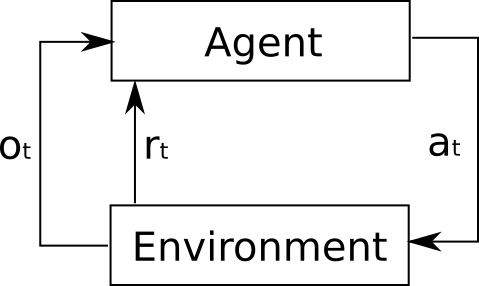
\includegraphics[width=0.9\columnwidth]{./Images/rl_agent.png}%
    \vfill\columnbreak	
	$a_i$: action\\
	$o_i$: observation\\
	$r_i$: reward
\end{multicols}

\end{frame}
\clearpage

%%%%%%%%%%%%%%%%%%%%%%%
%% Folie             %%
%%%%%%%%%%%%%%%%%%%%%%%
\begin{frame}
    \frametitle{Reinforcement Learning (RL)}

\begin{PraesentationAufzaehlung}
	\item Model-free RL\\
	Observations of the environment map directly to values or actions
	\item Model-based RL\\
	-- Uses an internal model to reason about the future\\
	-- Agent can avoid adverse consequences of trial-and error in\\
	\hspace{5mm} real environments\\
	-- Better generalization across states%\\
	%-- Scale performance by increasing amount of internal simulations
\end{PraesentationAufzaehlung}

\end{frame}
\clearpage

%%%%%%%%%%%%%%%%%%%%%%%
%% Folie             %%
%%%%%%%%%%%%%%%%%%%%%%%
\begin{frame}
    \frametitle{Drawbacks of Model Based RL}


\begin{PraesentationAufzaehlung}
    \item The performance of model-based agents suffer if the model is inperfect\\
    \item It is not always possible to get an exact transition model
exact transition model is available
\end{PraesentationAufzaehlung}

$\rightarrow$ Combine model free and model based RL to get an agent\\
\hspace{8mm} which is robost against model imperfections.
\end{frame}
\clearpage

%%%%%%%%%%%%%%%%%%%%%%%
%% Folie             %%
%%%%%%%%%%%%%%%%%%%%%%%
%\begin{frame}
%    \frametitle{What we want}

%\begin{multicols}{2}

%	Combine model free and model based RL to get an agent which is robost against model imperfections
%    \vfill\columnbreak
%	\begin{center}
%    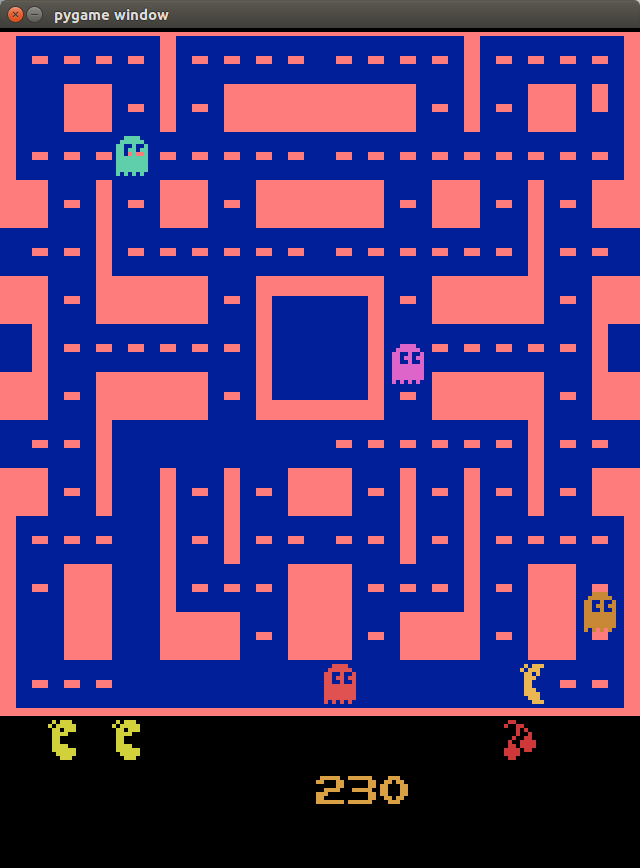
\includegraphics[height=.6\textheight]{./Images/screenshot_ghost.png}%
%	\end{center}
%\end{multicols}

	%We want an agent who learn to interpret predictions from a learned environment model to construct plans in arbitrary ways, by using the predictions as additional context in the deep policy network\\
%\end{frame}
%\clearpage



%%%%%%%%%%%%%%%%%%%%%%%
%% Folie             %%
%%%%%%%%%%%%%%%%%%%%%%%
%\begin{frame}
%    \frametitle{Goals}

%\begin{PraesentationAufzaehlung}
%    \item Working Implementation of I2A in pytorch
%\end{PraesentationAufzaehlung}

%\end{frame}
%\clearpage

%%%%%%%%%%%%%%%%%%%%%%%%%%%%%%%%%%%%%%%%%%%%%%%%%%%%%  
 % FOLIENSTIL: Weisse Schrift auf blauem Grund 
\PraesentationMasterWeissBlau 
\begin{frame} 
    \PraesentationUeberschriftZweizeilig{Imagination-Augmented Agent (I2A)}{Weber et al. (2017)}

\end{frame} 

\PraesentationMasterStandard


%%%%%%%%%%%%%%%%%%%%%%%
%% Folie             %%
%%%%%%%%%%%%%%%%%%%%%%%
\begin{frame}
    \frametitle{Imagination-Augmented Agent (I2A)}

\begin{PraesentationAufzaehlung}
	\item Weber et al.(2017)
    \item Imagine the future and learn to do better actions based on the imagined future
    \item Combines model-free and model-based aspects
\end{PraesentationAufzaehlung}

\end{frame}
\clearpage

%%%%%%%%%%%%%%%%%%%%%%%%%%%%%%%%%%%%%%%%
%% Folie: Bilder                      %%
%%%%%%%%%%%%%%%%%%%%%%%%%%%%%%%%%%%%%%%%
\begin{frame}
    \frametitle{I2A Architecture}


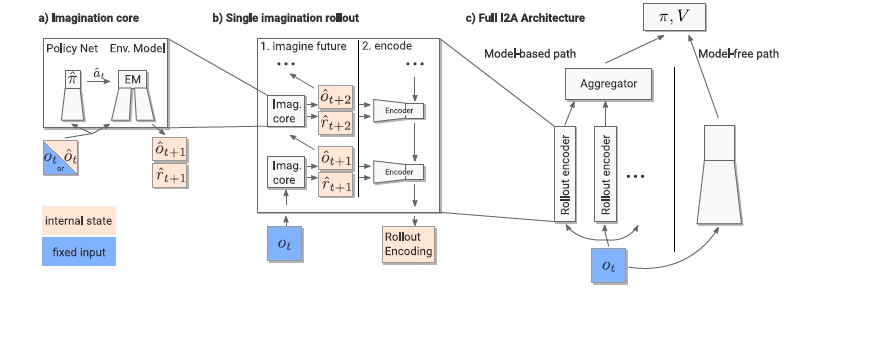
\includegraphics[width=\columnwidth]{./Images/i2a_architecture.png}%
\begin{PraesentationAufzaehlung}
\item Network architecture for deep reinforcement learning which combines model free and model based RL
\end{PraesentationAufzaehlung}
    
\end{frame}
\clearpage

%%%%%%%%%%%%%%%%%%%%%%%%%%%%%%%%%%%%%%%%
%% Folie: Bilder - Zweispaltige Seite %%
%%%%%%%%%%%%%%%%%%%%%%%%%%%%%%%%%%%%%%%%
\begin{frame}
    \frametitle{Training I2A}

\begin{multicols}{2}
	\begin{PraesentationAufzaehlung}
		\item Input:\\
		Observation $o_t$
		\item Output:\\
		Learned policy $\pi$ and value function $V$
		\item Train with Advantage-Actor-Critic (A2C)
	\end{PraesentationAufzaehlung}
    \vfill\columnbreak
	\begin{center}
    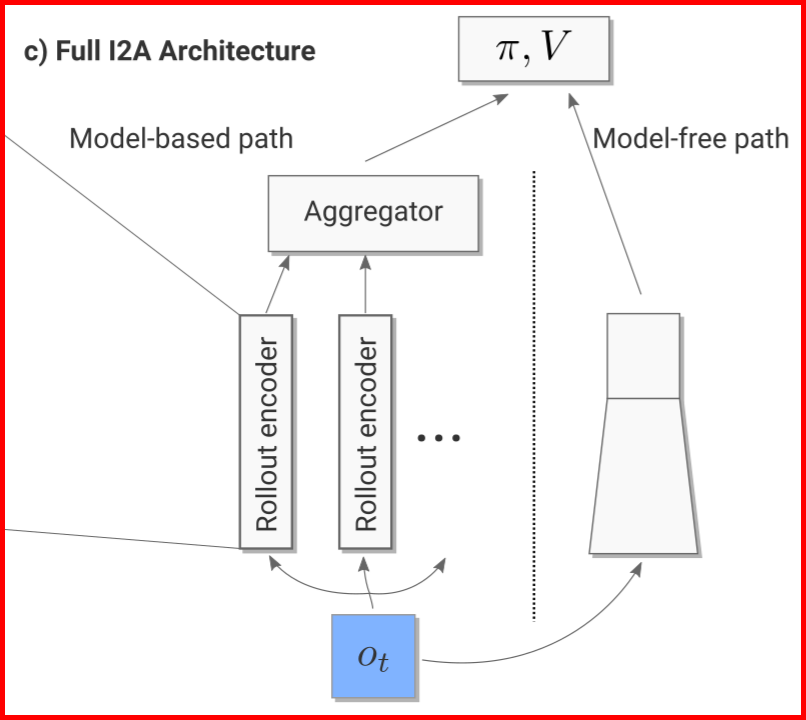
\includegraphics[width=\columnwidth]{./Images/i2a_a2c.png}%
	\end{center}
\end{multicols}
    
\end{frame}
\clearpage

%%%%%%%%%%%%%%%%%%%%%%%
%% Folie             %%
%%%%%%%%%%%%%%%%%%%%%%%
\begin{frame}
    \frametitle{Advantage-Actor-Critic (A2C)}

\begin{PraesentationAufzaehlung}
    \item Actor	learns policy function $\mathnormal{\pi(s, a, \theta)}$:\\
	Controls how the agent acts\\
	Policy update:
	\begin{equation}
	\mathnormal{\nabla \theta = \alpha \nabla_\theta (log \pi_\theta (s, a)) q_w (s, a)}
	\end{equation}	
	\item Critic learns value function $\mathnormal{V(s, a, w)}$:\\
	Messures how good a choosen actions is\\
	Value update:
	\begin{equation}
	\mathnormal{
	\nabla w = \beta (R(s, a) + \gamma q_w(s_{t+1}, a_{t+1}) - q_w(s_t, a_t)) \nabla_w q_w(s_t, a_t)}
	\end{equation}
\end{PraesentationAufzaehlung}

\end{frame}
\clearpage


%%%%%%%%%%%%%%%%%%%%%%%%%%%%%%%%%%%%%%%%
%% Folie: Bilder                      %%
%%%%%%%%%%%%%%%%%%%%%%%%%%%%%%%%%%%%%%%%
\begin{frame}
    \frametitle{I2A Architecture - Model Free Path}


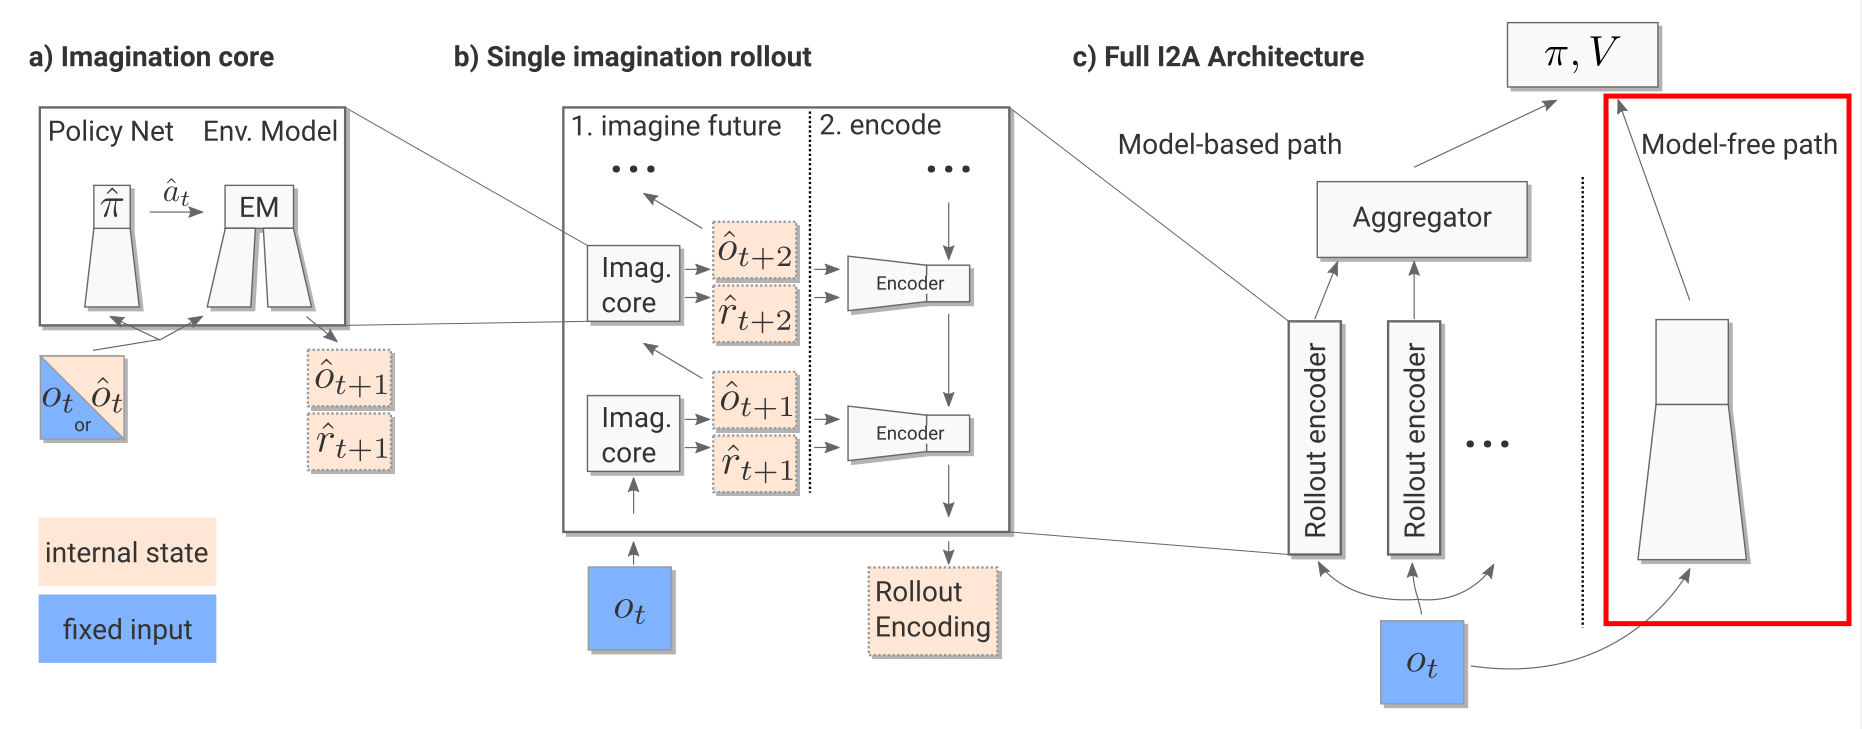
\includegraphics[width=\columnwidth]{./Images/i2a_all_model_free_path.png}%

\begin{PraesentationAufzaehlung}
	\item CNN Layers followed by Fully Connected Layers as usually used for Reinforcement Learning
\end{PraesentationAufzaehlung}

\end{frame}
\clearpage

%%%%%%%%%%%%%%%%%%%%%%%%%%%%%%%%%%%%%%%%
%% Folie: Bilder - Zweispaltige Seite %%
%%%%%%%%%%%%%%%%%%%%%%%%%%%%%%%%%%%%%%%%
%\begin{frame}
%    \frametitle{I2A Architecture - Model Free Path}

%\begin{multicols}{2}
%	\begin{PraesentationAufzaehlung}
%		\item 
%	\end{PraesentationAufzaehlung}
%    \vfill\columnbreak
%	\begin{center}
%    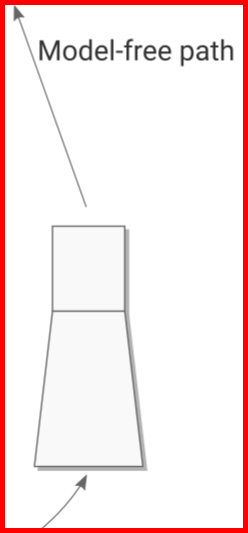
\includegraphics[height=.5\textheight]{./Images/i2a_model_free_path.png}%
%	\end{center}
%\end{multicols}
%    
%\end{frame}
%\clearpage


%%%%%%%%%%%%%%%%%%%%%%%%%%%%%%%%%%%%%%%%
%% Folie: Bilder                      %%
%%%%%%%%%%%%%%%%%%%%%%%%%%%%%%%%%%%%%%%%
\begin{frame}
    \frametitle{I2A Architecture - Model Based Path}


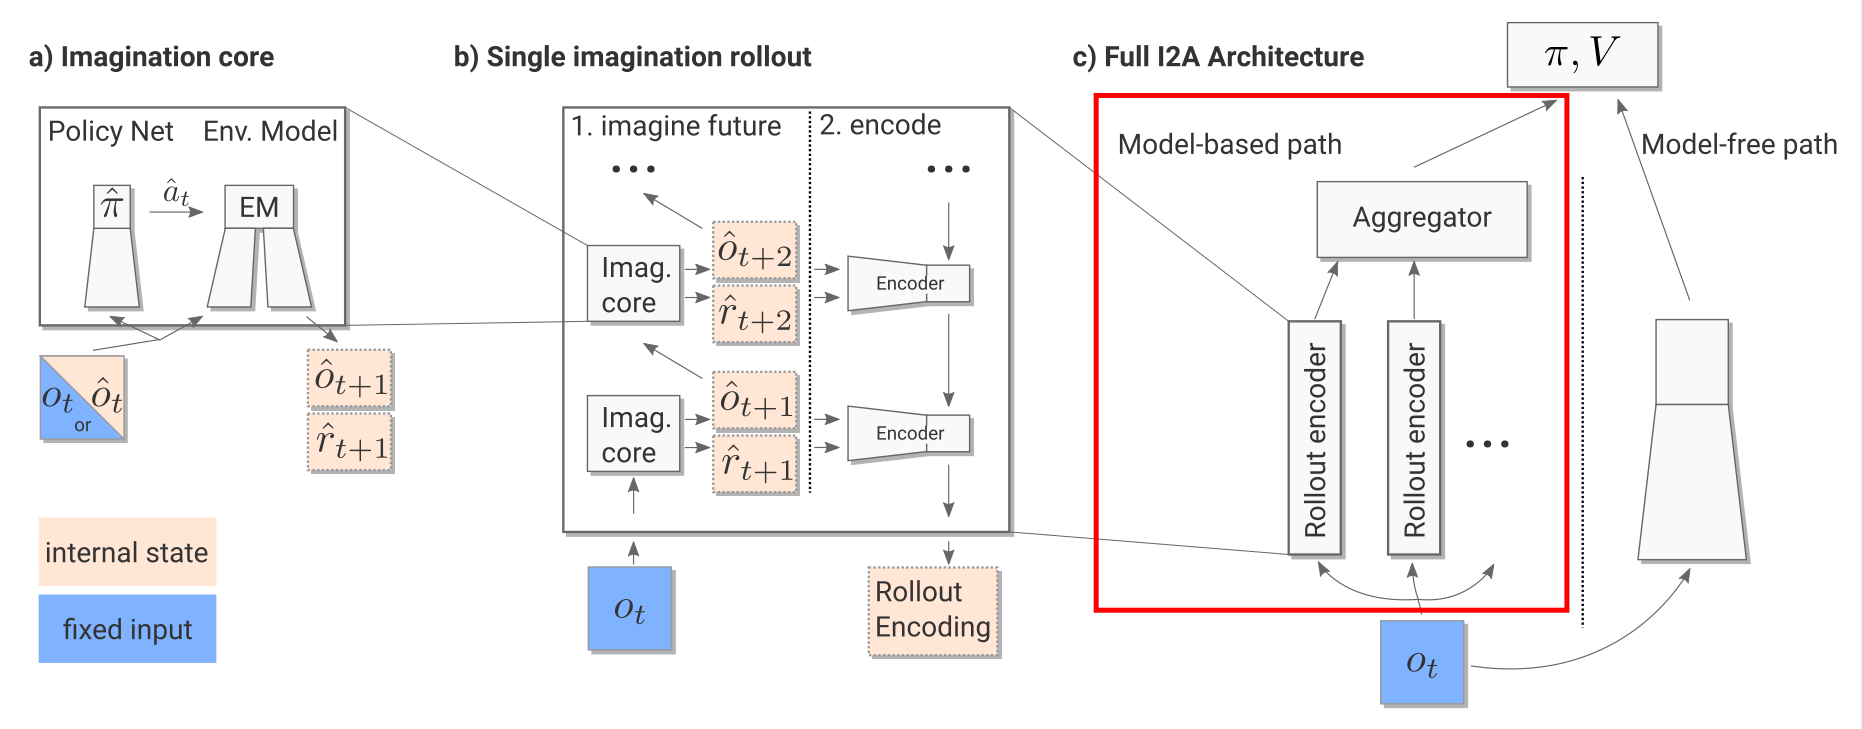
\includegraphics[width=\columnwidth]{./Images/i2a_all_model_based_path.png}%

\begin{PraesentationAufzaehlung}
	\item Imagine the future based on a model of the environment and use this information for decision making
\end{PraesentationAufzaehlung}
    
\end{frame}
\clearpage

%%%%%%%%%%%%%%%%%%%%%%%%%%%%%%%%%%%%%%%%
%% Folie: Bilder - Zweispaltige Seite %%
%%%%%%%%%%%%%%%%%%%%%%%%%%%%%%%%%%%%%%%%
\begin{frame}
    \frametitle{I2A Architecture - Model Based Path}

\begin{multicols}{2}
	\begin{PraesentationAufzaehlung}
	    \item Rollout encoder:\\
		For each action the agent can take, 
		imagine the future% and learn relevent information that can happen
		\item Aggregator: \\
		Concatinate all action rollouts
	\end{PraesentationAufzaehlung}
    \vfill\columnbreak
	\begin{center}
    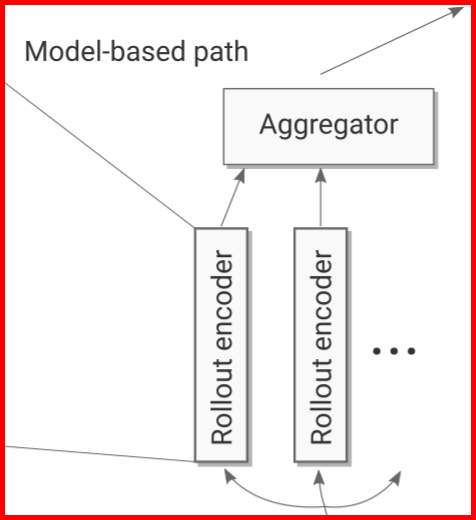
\includegraphics[height=.5\textheight]{./Images/i2a_model_based.png}%
	\end{center}
\end{multicols}
    
\end{frame}
\clearpage



%%%%%%%%%%%%%%%%%%%%%%%%%%%%%%%%%%%%%%%%
%% Folie: Bilder                      %%
%%%%%%%%%%%%%%%%%%%%%%%%%%%%%%%%%%%%%%%%
\begin{frame}
    \frametitle{I2A Architecture - Imagination Rollout}


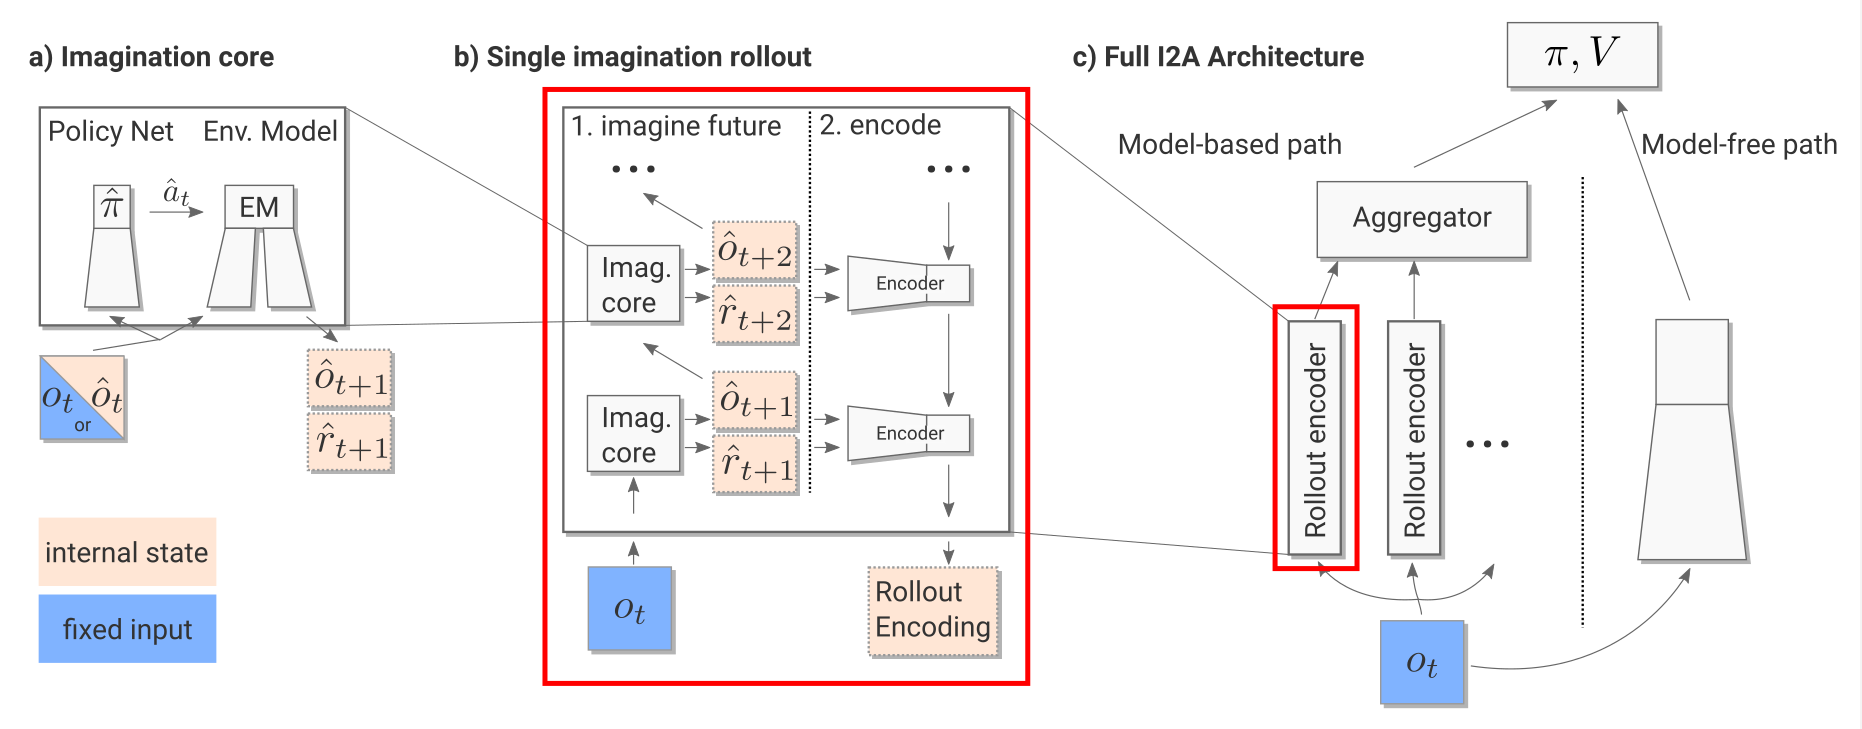
\includegraphics[width=\columnwidth]{./Images/i2a_all_imagination_rollout.png}%

\begin{PraesentationAufzaehlung}
	\item Predict what will happen in the future
\end{PraesentationAufzaehlung}
    
\end{frame}
\clearpage


%%%%%%%%%%%%%%%%%%%%%%%%%%%%%%%%%%%%%%%%
%% Folie: Bilder - Zweispaltige Seite %%
%%%%%%%%%%%%%%%%%%%%%%%%%%%%%%%%%%%%%%%%
\begin{frame}
    \frametitle{I2A Architecture - Imagination Future}

\begin{multicols}{2}
	\begin{PraesentationAufzaehlung}
		\item Input:\\
		observation $o_t$ and start action $a$
		\item Output:\\
		n imagined trajectories ($o_{t+i}, r_{t+i}$ for $i = 0, ..., n$)
	\end{PraesentationAufzaehlung}
    \vfill\columnbreak
	\begin{center}
    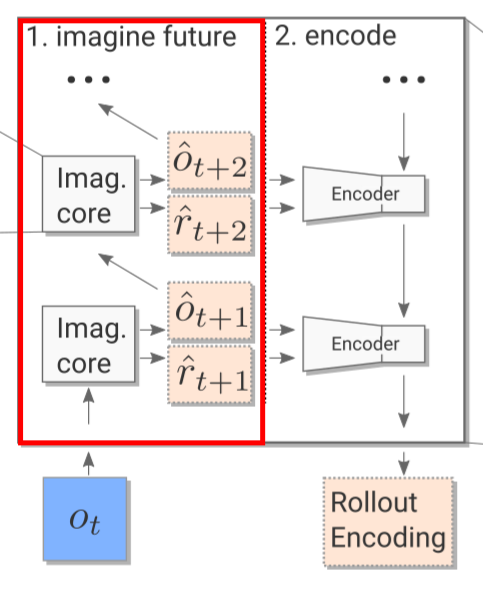
\includegraphics[height=.5\textheight]{./Images/imagine_future.png}%
	\end{center}
\end{multicols}
    
\end{frame}
\clearpage

%%%%%%%%%%%%%%%%%%%%%%%%%%%%%%%%%%%%%%%%
%% Folie: Bilder - Zweispaltige Seite %%
%%%%%%%%%%%%%%%%%%%%%%%%%%%%%%%%%%%%%%%%
\begin{frame}
    \frametitle{I2A Architecture - Encoder}

\begin{multicols}{2}
	\begin{PraesentationAufzaehlung}
		\item CNN Network followed by an LSTM Network
		\item Learns useful information from the rollout trajectories
	\end{PraesentationAufzaehlung}
    \vfill\columnbreak
	\begin{center}
    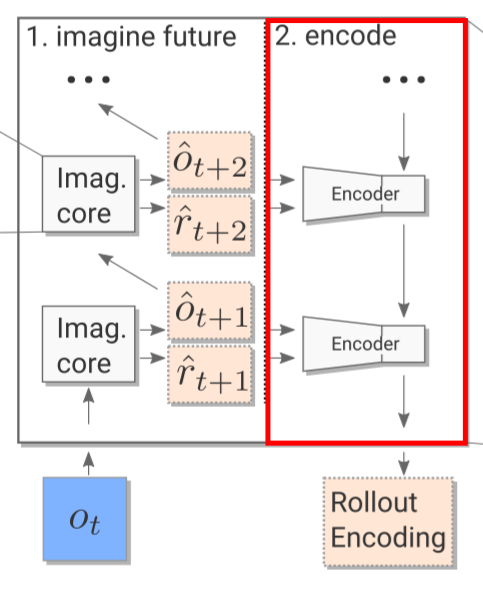
\includegraphics[height=.5\textheight]{./Images/encoder.png}%
	\end{center}
\end{multicols}
    
\end{frame}
\clearpage

%%%%%%%%%%%%%%%%%%%%%%%%%%%%%%%%%%%%%%%%
%% Folie: Bilder                      %%
%%%%%%%%%%%%%%%%%%%%%%%%%%%%%%%%%%%%%%%%
\begin{frame}
    \frametitle{I2A Architecture - Imagination Core}


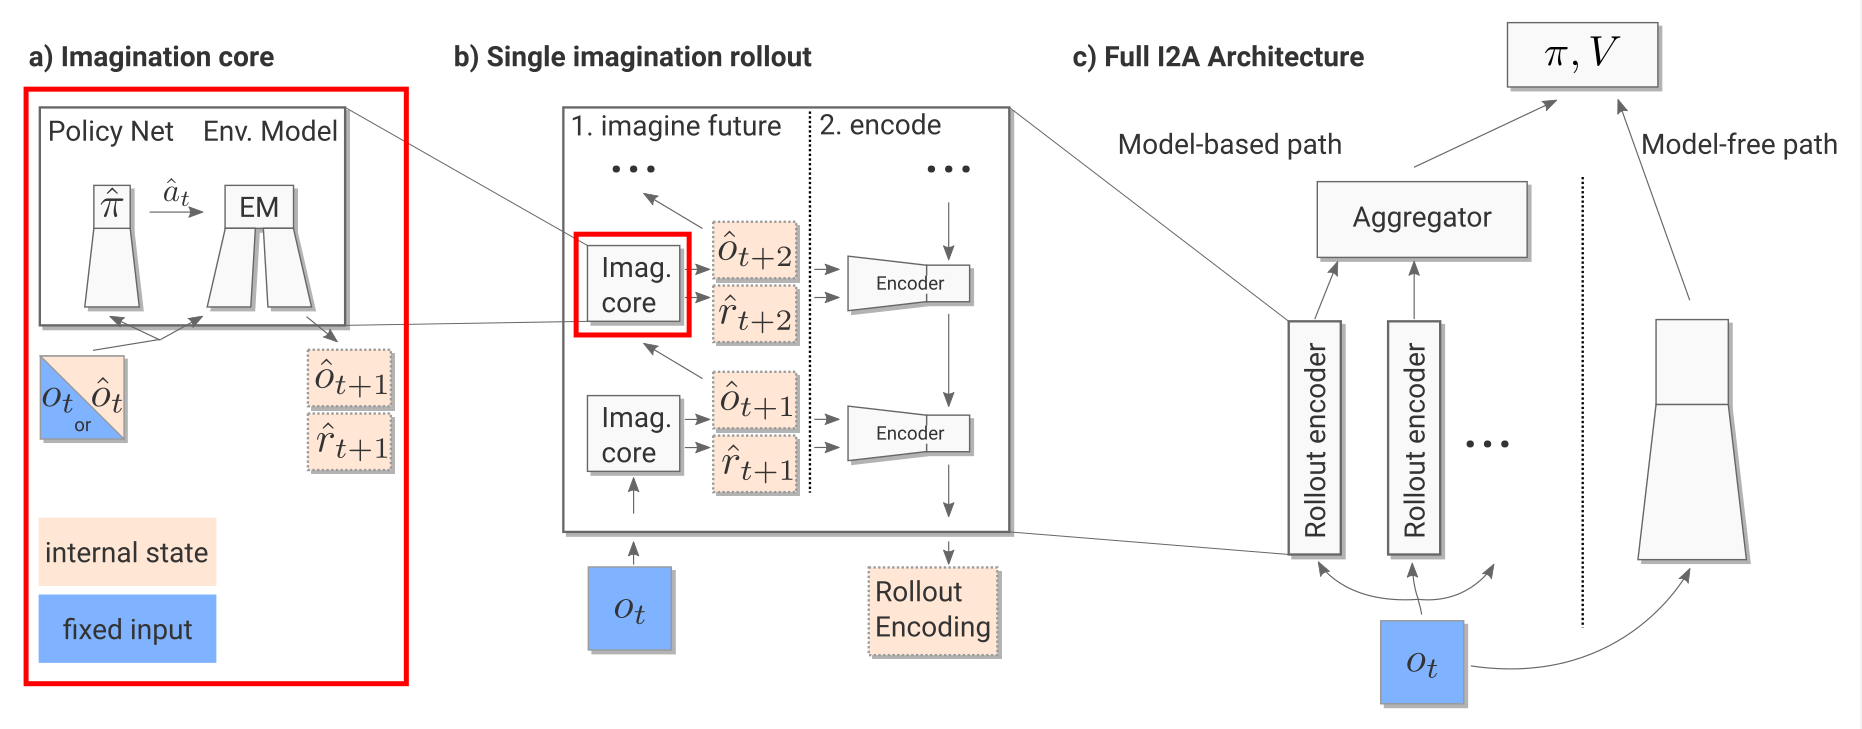
\includegraphics[width=\columnwidth]{./Images/i2a_all_imagination_core.png}%

\begin{PraesentationAufzaehlung}
	\item Imagine the next observation $\hat{o}_{t+i}$ and next reward $\hat{r}_{t+i}$ given observation $\hat{o}_{t+i-1}$
\end{PraesentationAufzaehlung}
\end{frame}
\clearpage


%%%%%%%%%%%%%%%%%%%%%%%%%%%%%%%%%%%%%%%%
%% Folie: Bilder - Zweispaltige Seite %%
%%%%%%%%%%%%%%%%%%%%%%%%%%%%%%%%%%%%%%%%
%\begin{frame}
%    \frametitle{I2A Architecture - Imagination Core}

%\begin{multicols}{2}
%	\begin{PraesentationAufzaehlung}
%		\item Imaginate the next observation $o_{t+i}$ and next reward $r_{t+i}$ given observation $o_t$
%	\end{PraesentationAufzaehlung}
%    \vfill\columnbreak
%	\begin{center}
%    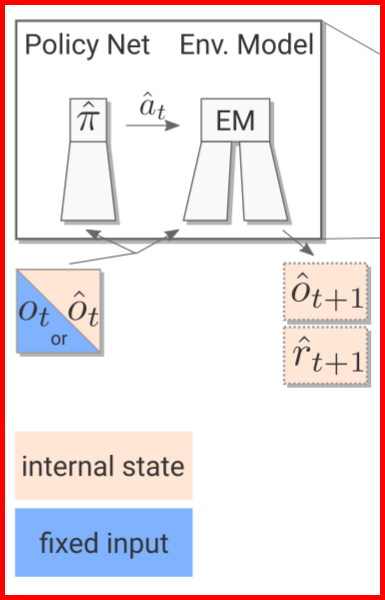
\includegraphics[height=0.5\textheight]{./Images/i2a_imagination_core.png}%
%	\end{center}
%\end{multicols}
    
%\end{frame}
%\clearpage

%%%%%%%%%%%%%%%%%%%%%%%%%%%%%%%%%%%%%%%%
%% Folie: Bilder - Zweispaltige Seite %%
%%%%%%%%%%%%%%%%%%%%%%%%%%%%%%%%%%%%%%%%
\begin{frame}
    \frametitle{Imagination Core - Policy Network}

\begin{multicols}{2}
	\begin{PraesentationAufzaehlung}
	    \item Policy network $\hat{\pi}$ decides the next action $a_t$
		\item Distillation loss\\
		Make $\hat{\pi}$ (rollout policy) and $\pi$ (i2a policy) similar\\
	\end{PraesentationAufzaehlung}
    \vfill\columnbreak
	\begin{center}
    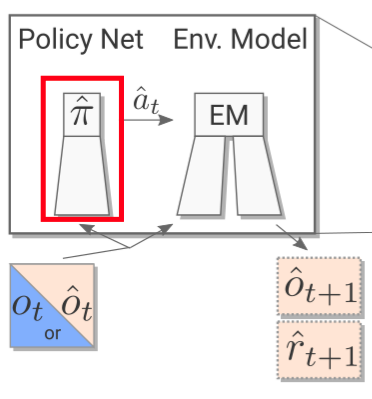
\includegraphics[height=0.35\textheight]{./Images/policy_net.png}%
	\end{center}
\end{multicols}
\begin{PraesentationAufzaehlung}	    
	\item Cross Entropy between $\pi$ and $\hat{\pi}$\\
	\begin{equation}
		\mathnormal{
		l_{dist}(\pi, \hat{\pi})(o_t) = \lambda_{dist} \sum_a \pi(a | o_t) log \hat{\pi}(a|o_t)
		}
	\end{equation}
\end{PraesentationAufzaehlung}
    
\end{frame}
\clearpage




%%%%%%%%%%%%%%%%%%%%%%%%%%%%%%%%%%%%%%%%%%%%%%%%%%%%%  
 % FOLIENSTIL: Weisse Schrift auf blauem Grund 
\PraesentationMasterWeissBlau 
\begin{frame} 
    \frametitle{Environment Model (EM)}
\end{frame}

\PraesentationMasterStandard

%%%%%%%%%%%%%%%%%%%%%%%%%%%%%%%%%%%%%%%%
%% Folie: Bilder - Zweispaltige Seite %%
%%%%%%%%%%%%%%%%%%%%%%%%%%%%%%%%%%%%%%%%
\begin{frame}
    \frametitle{Environment Model (EM)}

\begin{multicols}{2}
	\begin{PraesentationAufzaehlung}
		\item Imagine what will happen if we are in state $o_t$ and do action $a_t$
	\end{PraesentationAufzaehlung}
    \vfill\columnbreak
	\begin{center}
    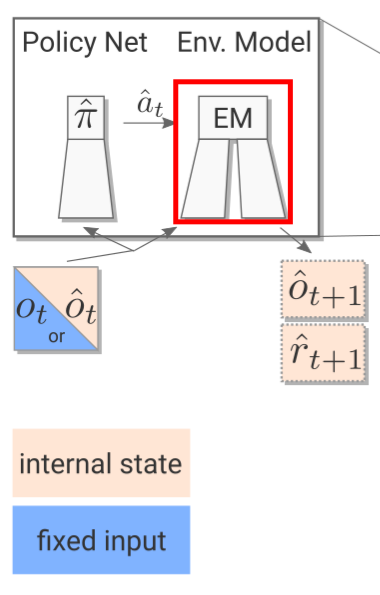
\includegraphics[height=0.5\textheight]{./Images/environment_model.png}%
	\end{center}
\end{multicols}
    
\end{frame}
\clearpage


%%%%%%%%%%%%%%%%%%%%%%%%%%%%%%%%%%%%%%%%
%% Folie: Bilder - Zweispaltige Seite %%
%%%%%%%%%%%%%%%%%%%%%%%%%%%%%%%%%%%%%%%%
\begin{frame}
    \frametitle{Environment Model Architecture}

\begin{multicols}{2}
	\begin{PraesentationAufzaehlung}
		\item Input:\\
		-- Stack of last 3 observations\\
		-- Action as one hot vector\\
		\item Trained with trajectories generated from a pretrained a2c policy
	\end{PraesentationAufzaehlung}
    \vfill\columnbreak
	\begin{center}
    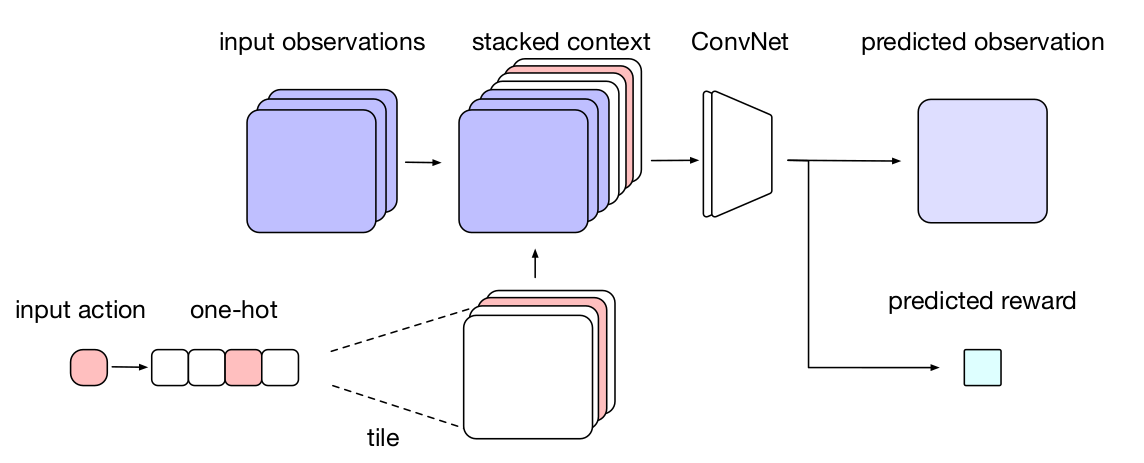
\includegraphics[width=\columnwidth]{./Images/environment_model_architecture.png}%
	\end{center}
\end{multicols}
    
\end{frame}
\clearpage




%%%%%%%%%%%%%%%%%%%%%%%%%%%%%%%%%%%%%%%%
%% Folie: Bilder - Zweispaltige Seite %%
%%%%%%%%%%%%%%%%%%%%%%%%%%%%%%%%%%%%%%%%
\begin{frame}
    \frametitle{Training Environment Model}

\begin{PraesentationAufzaehlung}
	\item Train similar to Autoencoder
	\item Maximize the log likelihood of the probability $p(o_t | a_{t-1}, o_{t-1})$
	\item Loss:\\
	\begin{equation}
	\mathnormal{
	env_{loss} = log p(o_t | a_{t-1}, o_{t-1})}
	\end{equation}	
	\item Image can be seen as Bernoulli distribution $p(o_t | a_{t-1}, o_{t-1})$
	\begin{equation}
	\mathnormal{
	env_{loss} = Binary Cross Entropy(predicted\_image, true\_images)
	}
	\end{equation}
\end{PraesentationAufzaehlung}
    
\end{frame}
\clearpage


%%%%%%%%%%%%%%%%%%%%%%%%%%%%%%%%%%%%%%%%%%%%%%%%%%%%%  
 % FOLIENSTIL: Weisse Schrift auf blauem Grund 
\PraesentationMasterWeissBlau 
\begin{frame} 
    \frametitle{MiniPacman}
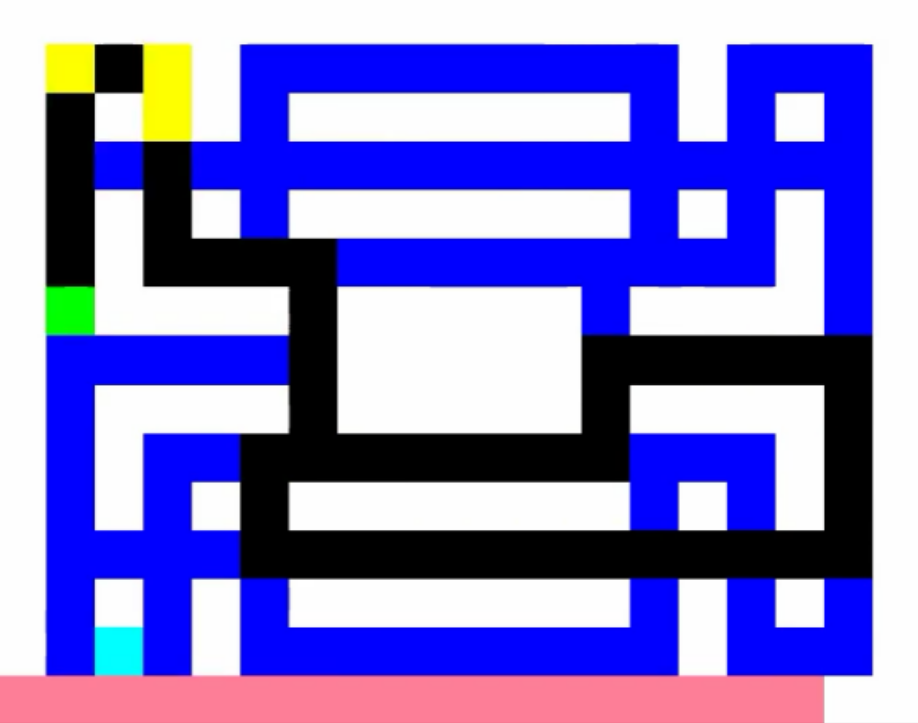
\includegraphics[height=0.5\textheight]{./Images/mini_pacman.png}%
\end{frame} 

\PraesentationMasterStandard

%%%%%%%%%%%%%%%%%%%%%%%%%%%%%%%%%%%%%%%%
%% Folie: Bilder - Zweispaltige Seite %%
%%%%%%%%%%%%%%%%%%%%%%%%%%%%%%%%%%%%%%%%
\begin{frame}
    \frametitle{MiniPacman}

\begin{PraesentationAufzaehlung}
	\item I2A Model Based Path expensive to train
	\item Uses 15 x 19 Grid World version of Pacman
	\item Makes vision problem easier but preserves the reinforcement learning problem
	\item MiniPacman can be played in different modes
\end{PraesentationAufzaehlung}
    
\end{frame}
\clearpage

%%%%%%%%%%%%%%%%%%%%%%%%%%%%%%%%%%%%%%%%
%% Folie: Bilder - Zweispaltige Seite %%
%%%%%%%%%%%%%%%%%%%%%%%%%%%%%%%%%%%%%%%%
\begin{frame}
    \frametitle{MiniPacman -- Hunt}

Rewards:

	\hspace{-4mm}
	\begin{tabular}{ p{7cm}  r }
 	At each step & 0 \\
  	Eating food & 0 \\
	Eating power pill & 1\\
	Eating ghost & 10\\
	Killed by ghost & -20\\
	\end{tabular}
    
\end{frame}
\clearpage


%%%%%%%%%%%%%%%%%%%%%%%%%%%%%%%%%%%%%%%%
%% Folie: Bilder - Zweispaltige Seite %%
%%%%%%%%%%%%%%%%%%%%%%%%%%%%%%%%%%%%%%%%
\begin{frame}
    \frametitle{EnvironmentModel Hunt Demo}
    
\end{frame}
\clearpage

%%%%%%%%%%%%%%%%%%%%%%%%%%%%%%%%%%%%%%%%
%% Folie: Bilder - Zweispaltige Seite %%
%%%%%%%%%%%%%%%%%%%%%%%%%%%%%%%%%%%%%%%%
\begin{frame}
    \frametitle{Implementation I2A}

\begin{PraesentationAufzaehlung}
	\item Based on A2C implementation of Kostrikov \url{https://github.com/ikostrikov/pytorch-a2c-ppo-acktr} 
	\item Pytorch as Deep Learning Library
	\item Environment Model and I2A implementation will be published on github
\end{PraesentationAufzaehlung}
    
\end{frame}
\clearpage


%%%%%%%%%%%%%%%%%%%%%%%%%%%%%%%%%%%%%%%%
%% Folie: Bilder - Zweispaltige Seite %%
%%%%%%%%%%%%%%%%%%%%%%%%%%%%%%%%%%%%%%%%
\begin{frame}
    \frametitle{I2A MiniPacman Hunt Results}

\begin{multicols}{2}
	\begin{center}
    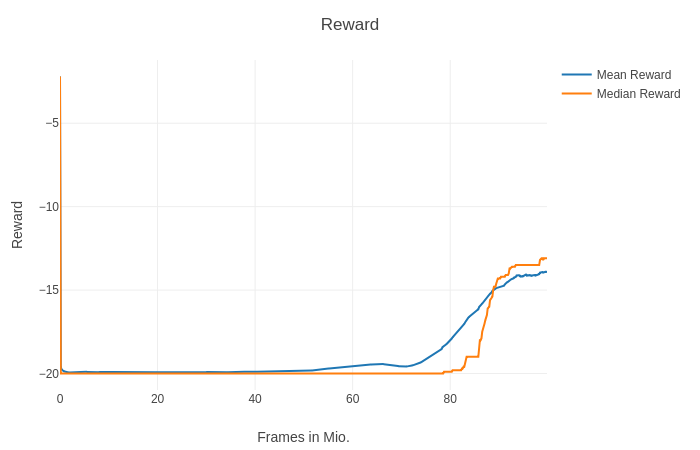
\includegraphics[width=\columnwidth]{./Images/a2c_hunt_reward.png}\\
	A2C Hunt Reward Training Curve (100 mio frames)
	\end{center}
    \vfill\columnbreak
	\begin{center}
    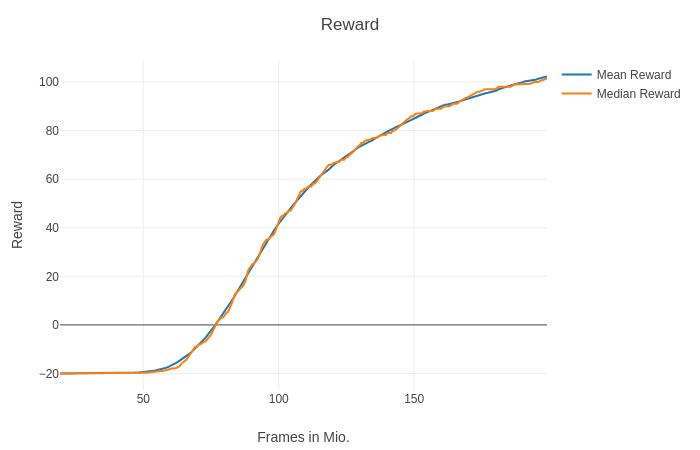
\includegraphics[width=\columnwidth]{./Images/i2a_hunt_reward_mean_and_median.png}\\
	I2A Hunt Reward Training Curve (200 mio frames)
	\end{center}
\end{multicols}
\end{frame}
\clearpage

%%%%%%%%%%%%%%%%%%%%%%%%%%%%%%%%%%%%%%%%
%% Folie: Bilder - Zweispaltige Seite %%
%%%%%%%%%%%%%%%%%%%%%%%%%%%%%%%%%%%%%%%%
\begin{frame}
    \frametitle{I2A Hunt Demo}
    
\end{frame}
\clearpage


%%%%%%%%%%%%%%%%%%%%%%%%%%%%%%%%%%%%%%%%
%% Folie: Bilder - Zweispaltige Seite %%
%%%%%%%%%%%%%%%%%%%%%%%%%%%%%%%%%%%%%%%%
\begin{frame}
    \frametitle{Questions?}
    
\end{frame}
\clearpage



